%

\documentclass[UTF8]{ctexbook}

\ctexset{
    part/number = \chinese{part}% 用于解决 part 的标号不显示问题
}
\usepackage{hyperref}% 超链接
\hypersetup{
    colorlinks=false,% 去掉超链接颜色
    pdfborder=0 0 0% 取消超链接的边框
}
\usepackage{graphicx}% 图片管理
\graphicspath{{images/}}% 设置图片搜索路径
\usepackage{float,varwidth}% 浮动体
\usepackage{booktabs}% 三线表
\usepackage{tabularx}% 让表格自适应宽度与自动换行
\newcolumntype{Y}{>{\centering\arraybackslash}X}% 定义自适应列的居中格式 Y, 用 X 为左对齐(自适应列)
\usepackage{fancyhdr}% 页眉设置
\usepackage{xcolor}% 颜色宏包
\usepackage{listings}% 代码高亮
\definecolor{codegreen}{rgb}{0,0.6,0}
\definecolor{codegray}{rgb}{0.5,0.5,0.5}
\definecolor{codepurple}{rgb}{0.58,0,0.82}
\definecolor{backcolour}{rgb}{0.95,0.95,0.92}
\lstset{
    commentstyle=\color{codegreen},
    keywordstyle=\color{magenta},
    stringstyle=\color{codepurple},
    basicstyle=\footnotesize,% 代码字体大小
    breakatwhitespace=false,% 是否只在空白字符处断行
    breaklines=true,% 自动断行
    captionpos=b,% 标题位置为 bottom
    keepspaces=true,
    numbers=left,% 行号的位置
    numbersep=5pt,% 行号与代码的距离
    numberstyle=\tiny\color{codegray},% 行号样式
    stepnumber=2,% 隔行显示行号
    showspaces=false,
    showstringspaces=false,
    showtabs=false,
    tabsize=2
}

\begin{document}
  \chapter{开发流程}
    \label{chap:开发流程}

  \section{总体开发流程}
    \label{sec:总体开发流程}
      本次的项目采用 AngularJS 框架开发,AngularJS 项目一般由入口页、模板、控制器、路由控制以及静态资源几大模块构成。大体而流程是: 路由配置 -> 模板设计 -> 数据构造 -> 控制器配置,这些模块的编写没有严格的顺序,模块间是由关联的,因此,改动了一个模块,其他关联的而模块都要跟着改动,下面就简单介绍一下各流程所做的工作。

    \subsection{项目结构}
      \label{subsec:项目结构}
        整个项目的目录结构及如下:
                         aystore
                          |
                          |---css/ // CSS 静态资源
                          |    |---artdetail.css
                          |    |---artlist.css
                          |    |---botbar.css
                          |    ...
                          |
                          |---img/ // 主要是一些图标
                          |    |---alipay.png
                          |    |---home.jpg
                          |    ...
                          |
                          |---less // less 文件,用于编译成 CSS
                          |---node_modules // 项目用到的模块, 如 AngularJS
                          |---res // 存放一些资料,如设计图,方案规划等,不属于项目
                          |---tpl // 模板文件
                          |    |---artdetail.html
                          |    |---ayculture.html
                          |    |---pay.html
                          |    ...
                          |---app.js   // 控制器入口,路由控制,控制器代码
                          |---index.js // 视图入口,html 基本结构,静态资源的一次性引入
        \par
        css 目录是样式目录,用来控制页面的样式;img 目录放置了 html 文件中用到的所有的图标;less 目录是存放的 less 文件,要编译成 css 文件才能执行,我采用了 Sublime 的一个插件 Less2Css,使用时他会调用 lessc 引擎,在 Less 文件保存时可以自动将其编译为 css 文件到指定目录,非常高效。node_modules 文件夹存放了项目所需的库,由 npm 包管理工具下载的库或框架都放在 node_modules 文件夹下。res 文件夹存放了资料,例如项目规划、设计图等,不属于项目组成;tpl 文件夹存放了模板文件,对应于 MVC 模型中的 view, 由控制器控制路由与填充数据。入口页 index.html 负责引入页面的基本框架、静态资源以及视图入口。这是 SPA 应用的模式,详见 \ref{subsubsec:spa}。app.js 是控制逻辑的入口页,包含了路由的配置及各个模板的控制器。

    \subsection{路由配置}
      \label{subsec:路由配置}
        路由的机制我们在 \ref{subsubsec:ui_router_模块} 简要介绍过,我把项目中的路由划分为了两个部分,一个是包含底部菜单的路由,另一个是没有底部菜单的路由。有底部菜单的路由都设置成某个父路由的子路由,父路由的代码如下:
        \begin{lstlisting}
          $stateProvider
            .state('main', {
              url: '/main',
              templateUrl: "tpl/main.html",
              views: {
                '': {
                  templateUrl: "tpl/main.html"
                },
                'content@main': {
                   templateUrl: "tpl/home.html"
                },
                'botmenu@main': {
                   templateUrl: "tpl/botmenu.html"
                },
              }
            })
        \end{lstlisting}
          上面的代码是主路由(或者叫父路由)的配置,state() 方法的第一个参数为状态名,或者叫路由名; 第二个参数是一个对象,url 字段表示 "main" 这个路由的路径,templateUrl 表示显示的页面文件,此页面文件的作用是划分视图,这里划分为两个视图,一个对应主要内容,另一个对应底部菜单。继承了 "main" 这个路由的子路由继承了 "main" 的整个模板,包括底部菜单与内容部分,然后只需修改 content 的部分就可以实现子路由的视图。

    \subsection{模板与样式设计}
      \label{subsec:模板与样式设计}
        一个模板就是一个页面,只不过很简洁,只有关键的 html 代码,而没有外部文件引入、页面头的设置等,如图 \ref{fig:tpl1}, 这就是前面提到的 SPA (单页应用)的特性,详见 \ref{subsubsec:spa} 一节。
        \begin{figure}[H]
          \centering
          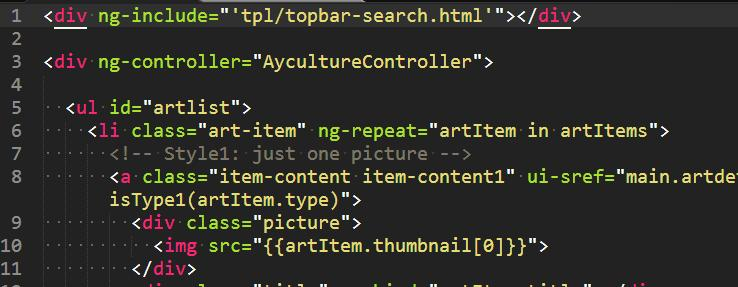
\includegraphics[width=8cm]{./img/tpl.jpg}
          \caption{简洁的模板页}
          \label{fig:tpl1}
        \end{figure}
        模板的主要作用是展现页面,因此要和配合 CSS 的控制。SPA 应用的样式需要考虑命名空间的问题,因为所有的 CSS 文件都是一次性引入的,如图 \ref{fig:css}
        \begin{figure}[H]
          \centering
          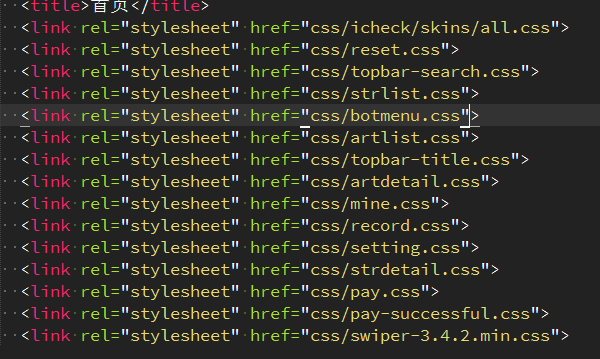
\includegraphics[width=10cm]{./img/css.png}
          \caption{一次性引入所有的 CSS 样式}
          \label{fig:css}
        \end{figure}
        我个人的处理方法是:对于每个 CSS 文件,用一个和文件名一样的容器把样式包裹起来,当然,我直接编辑的仍是 Less 文件,像这样 \ref{fig:wrapper},而且用 ID 而不是 Class 来确保唯一性, 让每个CSS 有自己的作用域,这个灵感来自于 AngularJS 的控制器的作用域,把每个模板的数据封闭起来,很好的避免了冲突。
        \begin{figure}[H]
          \centering
          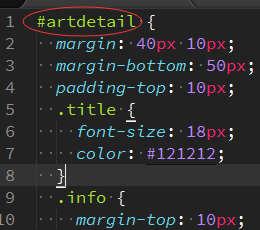
\includegraphics[width=5cm]{./img/wrapper.png}
          \caption{用 Wrapper 包裹起整个 Less 文件}
          \label{fig:wrapper}
        \end{figure}

    \subsection{数据与逻辑业务}
      \label{subsec:数据与逻辑业务}
        数据部分是前端设计中很重要的一环,个人认为,前端的设计大体分为两大块内容,一个是样式的设计,一个是数据与逻辑业务。好的样式设计需要花很长的时间,因为应用越精美,需要调的细节就越多,但 CSS 并不是一门语言,他只是个属性库而已,通过一点一点叠加样式实现想要的效果,没有深入的概念,没有更高的抽象的层次;而数据部分,更多地涉及逻辑,属于 JavaScript 部分,是编程,是语言,这就需要开发者有着很强的 JavaScript 语言基础,尤其是 DOM 和 BOM 对象,掌握一门语言是要花很长时间的,大量的而应用才能更深入的理解本质,例如 JavaScript 的一些核心概念:原型、继承、对象等,如果理解不够深入,编写的代码就可能冗杂、难以维护。尤其在用框架的时候,框架固然简单,可以大大简化代码,但是缺点是这是别人的东西,自己不理解原理,实现相同功能的 API 有很多,但其实用到的是同一段核心代码,此时与其去记忆那么多方法,不如深入挖掘代码,理解本质,这样才能走得更远。

    \subsection{控制器设计}
      \label{subsec:控制器设计}
        控制器的作用,个人通过写代码的理解,主要作用是指挥,指挥模型与模板,指挥数据朝哪走,例如:路由控制、请求控制,根据URL调用哪个页面以及获得 HTTP 请求后,把请求送给谁(某个服务)处理,控制器中不推荐写业务逻辑、数据的具体处理。
        \par
        控制器在两个地方设置,模板文件中的引入,用来控制作用范围,js 文件中的定义与具体逻辑实现。我的项目中,每个模板页的主要内容都用一个控制器包裹起来,如图 \ref{fig:ctrl},
        \begin{figure}[H]
          \centering
          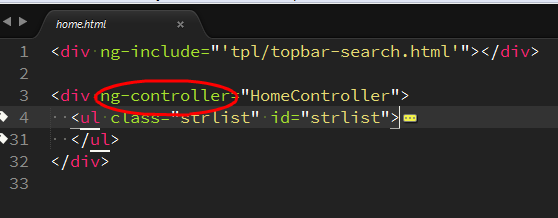
\includegraphics[width=8cm]{./img/ctrl.png}
          \caption{模板中的控制器声明 }
          \label{fig:ctrl}
        \end{figure}
        其他的地方是代码片段的包含,用其他的控制器设置,也就是说,控制器只是控制一部分 html 片段,让代码片段间的数据隔离,因此,一个页面是可以被多个控制器同时控制的,多个页面的某部分也可以由一个控制器来控制,例如底部菜单的部分,好几个页面都有,甚至有的页面一个控制器也没有,例如视图页,只放两行代码,用于模板的插入,此机制是由 ui-router 实现的,详见 \ref{subsubsec:ui_router_模块}。
        \par
        控制器的 js 代码放在了 app.js 文件中,,如图 \ref{fig:ctrl_js}
        \begin{figure}[H]
          \centering
          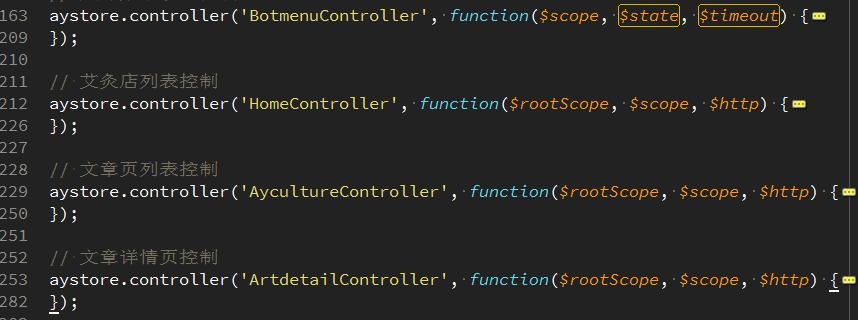
\includegraphics[width=12cm]{./img/ctrl_js.png}
          \caption{app.js 中的控制器}
          \label{fig:ctrl_js}
        \end{figure}
        此文件放置了所有的控制器代码以及路由配置,后面会一一讲到。

        \par
        以上的步骤没有严格而顺序,因为各部分会相互关联,例如:修改模板的 HTML 结构时,样式文件也要跟着修改很多,因此,各个过程几乎是同时进行的。接下来我就对每一页的技术与设计过程进行详细介绍。

  \section{home 页的设计}
    \label{sec:home_页的设计}

    \subsection{功能分析}
      \label{subsec:功能分析}
        首页的设计图 \ref{fig:home}:
        \begin{figure}[H]
          \centering
          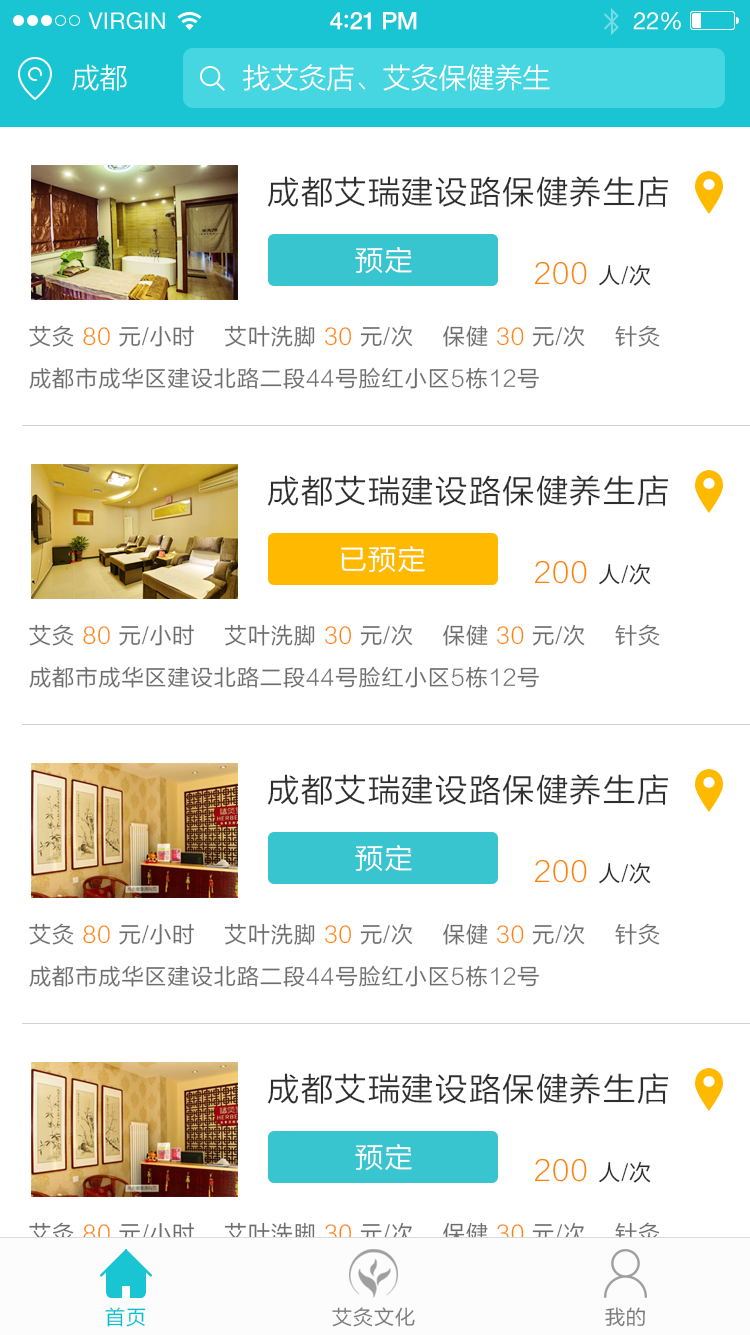
\includegraphics[width=8cm]{img/201705181050.jpg}
          \caption{首页设计图}
          \label{fig:home}
        \end{figure}
        首页主要实现如下功能:
        \begin{itemize}
          \item 地理定位
          \item 商城列表展现
          \item 商城搜索
        \end{itemize}

        \subsubsection{地理定位}
          \label{subsubsec:地理定位功能}
            首次进入商城,(todo)微信接口?还是自己写?应用会自动调用地理定位接口获取客户客户当前的位置,精确到县级,如:成华区,如果定位失败,则返回错误信息,位置自动设置为上一次的位置,并且提醒客户手动定位,点击左上方的按钮
            figtodo: 圈住左上方地理位置选择的图
            就会进入城市选择页,如下图所示:
            figtodo: 城市选择页
            然后就可以选择相应的城市或县区,为了更好地用户体验,如图,还设置了热门城市、最近选择的栏目。

        \subsubsection{列表展现}
          \label{subsubsec:列表展现}
            自动定位(或手动定位)好当前位置后,服务器会返回当前城市的保健店的列表,如图 todo 首页的设计图,简要地展示每个保健店的基本信息,如:店名、缩略图、艾灸床保健价格、其他服务与价格、详细地址以及右上角黄色的地理定位按钮,点击后会应用会打开地图接口,提供更好地体验,如下图:
            figtodo: 店的地图接口
            还有,如果一个店曾经预定过,则会以黄色的按钮提示已预订,点击预定按钮后就会进入店的详情页,展示店的详细信息以及进行预定操作。

        \subsection{商城搜索 todo: 待实现}
          \label{subsec:商城搜索_todo_待实现}
            如图figtodo: 首页设计图,还提供了搜索框,可以根据关键词搜索你想要的店,可以看到搜索框旁边没有搜索按钮,因为搜索是实时显示的,称为增量搜索,而且还采用了自动补全技术,根据最近的搜索关键词和列表加载时自动生成的关键词数据库进行模糊匹配,效果如下:设计非常人性化。
            figtodo: 搜索功能展示

    \subsection{地理定位功能 todo}
      \label{subsec:地理定位功能_todo}

    \subsection{搜索功能 todo}
      \label{subsec:搜索功能_todo}

    \subsection{列表展现}
      \label{subsec:列表展现}

        \subsubsection{数据设计}
          \label{subsubsec:数据设计}
            根据设计图 \ref{fig:home},列表中的每一项展示了如下的信息:
            \begin{itemize}
              \item 缩略图
              \item 店名
              \item 预定状态
              \item 艾灸保健价格
              \item 其他各项服务与价格
              \item 详细地址
            \end{itemize}
            于是我们可以构建如下的 JSON 数据,模拟从数据库提取的数据:
            \begin{lstlisting}
              [
                  {
                    "strId": "123",// 店的 ID
                    "strCity": "成都",// 城市
                    "strDistrict": "成华区",// 市区
                    "strThumbnail": "http://i2.muimg.com/589268/8aefeb670174ad96t.jpg",// 缩略图
                    "strName": "成都艾瑞建设路保健养生店",// 店名
                    "ordStatus": 0,// 预定状态,0:已预订,1:未预定
                    "strLink": "strlink/store1.html",// todo
                    "avgPrice": 200,// 艾灸服务价格
                    "srvInfo": "专业技术服务提供服务,智能艾灸床 5 张,艾灸、刮痧、洗脚、按摩、保健、亚健康、养生。",// 描述
                    "full": 0,// 是否满员
                    // 其他服务的信息
                    "strServices": [
                      {
                        "srvName": "艾灸",// 服务名
                        "srvPrice": 80,// 服务价格
                        "srvUnit": "元/小时"// 价格单位
                      },
                      {
                        "srvName": "艾叶洗脚",
                        "srvPrice": 30,
                        "srvUnit": "元/次"
                      },
                      {
                        "srvName": "针灸",
                        "srvPrice": "",
                        "srvUnit": ""
                      }
                    ],
                    "strMap": "",// todo
                    "strAddress": "建设北路二段44号脸红小区5栋12号"// 详细地址
                  },
                  {
                      "strId": "123",
                      "strCity": "成都",
                      "strDistrict": "成华区",
                      ...
                  },
                  ...
              ]
            \end{lstlisting}
            缩略图字段是调用的外部的链接,我把图片放到了专门的图片服务器上存储,这样可以节约服务器的空间,这样服务器上不需要再单独开辟一个文件夹盛放图片,也省去了给图片命名的麻烦,也能防止误删、图片文件夹改名的操作导致的图片链接失效。我采用的图片服务器是 “贴图库”,网址为:\url{http://www.tietuku.com/}, 网站虽然样式粗糙,但功能上考虑地很周到,例如可以给图片分组,方便管理,而且可以一键生成图片外链(包括缩略图),点击相应的按钮即可,如图 \ref{fig:tietuku}
            \begin{figure}[H]
              \centering
              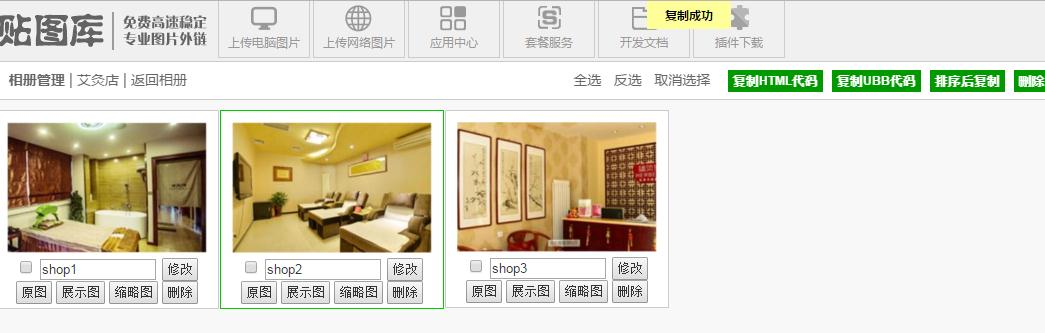
\includegraphics[width=10cm]{./img/tietuku.jpg}
              \caption{贴图库}
              \label{fig:tietuku}
            \end{figure}

        \subsubsection{dom 结构与 CSS 样式设计}
          \label{subsubsec:dom_结构与_css_样式设计}
            每一页的

        \subsubsection{控制器,路由}
          \label{subsubsec:控制器_路由}
            \paragraph{路由设计} 路由在前面讨论过,是指将 URL 与对应的模板关联起来,而且 AngularJS 支持模板继承与视图嵌套,在路由的配置上相当强大,详见 \ref{subsubsec:ui_router_模块} 一节。商城列表页的设计图 \ref{fig:home} 底部有控制菜单,根据前面的提到的,应该作为 "main" 路由的子路由,然后,只需修改 "content" 视图。代码如下:
            \begin{lstlisting}
              .state('main.home', {// 商城页视图
                url: '/home',
                views: {
                  'content@main': {
                     templateUrl: "tpl/home.html"
                  }
                }
              })
            \end{lstlisting}

            \paragraph{控制器设计}
            控制器的设计如前面提到的,分成两个部分,一个是模板中的引入,一个是 app.js 中的详细实现。这两个部分
            先来看模板部分,商城页部分主要是列表展现,列表的特点是重复,文章页也是类似,每个 item 都有相同的数据结构,在数据上是一个数组,因此需要用到 ng-repeat 命令,





















\end{document}
